\chapter{BLE-I2C Bridge}
\label{bleI2cBridge}

Das Sming verfügt über den Erweiterungsheader die Möglichkeit I2C Sensoren anzusprechen. Um diese Funktion zu nutzen muss die Firmware des Smings erweitert werden. Dies ist nicht Straight-Forward weil für die Entwicklung in C und das Deployment auf den NRF51 spezielle Hardware und Software erforderlich ist. Um dieses Problem zu umgehen wurde die BLE-I2C Bridge entwickelt. Sie soll dazu dienen, dass vom IoT-Gateway via Sming I2C Sensoren und Aktoren angesprochen werden können. Somit muss für einen neuen Sensor die Firmware der Smings nicht angerührt werden. Dafür muss aber das IoT-Gateway programmiert werden. Dieses lässt sich aber je nach Gateway Typ leicht über Ethernet oder USB programmieren. Auch die Softwareentwicklung in JavaScript sollte denn meisten Entwickler in der Informatik Branche weniger schwer fallen als dies bei C der Fall ist.

\begin{figure}[hbtp]
    \center
    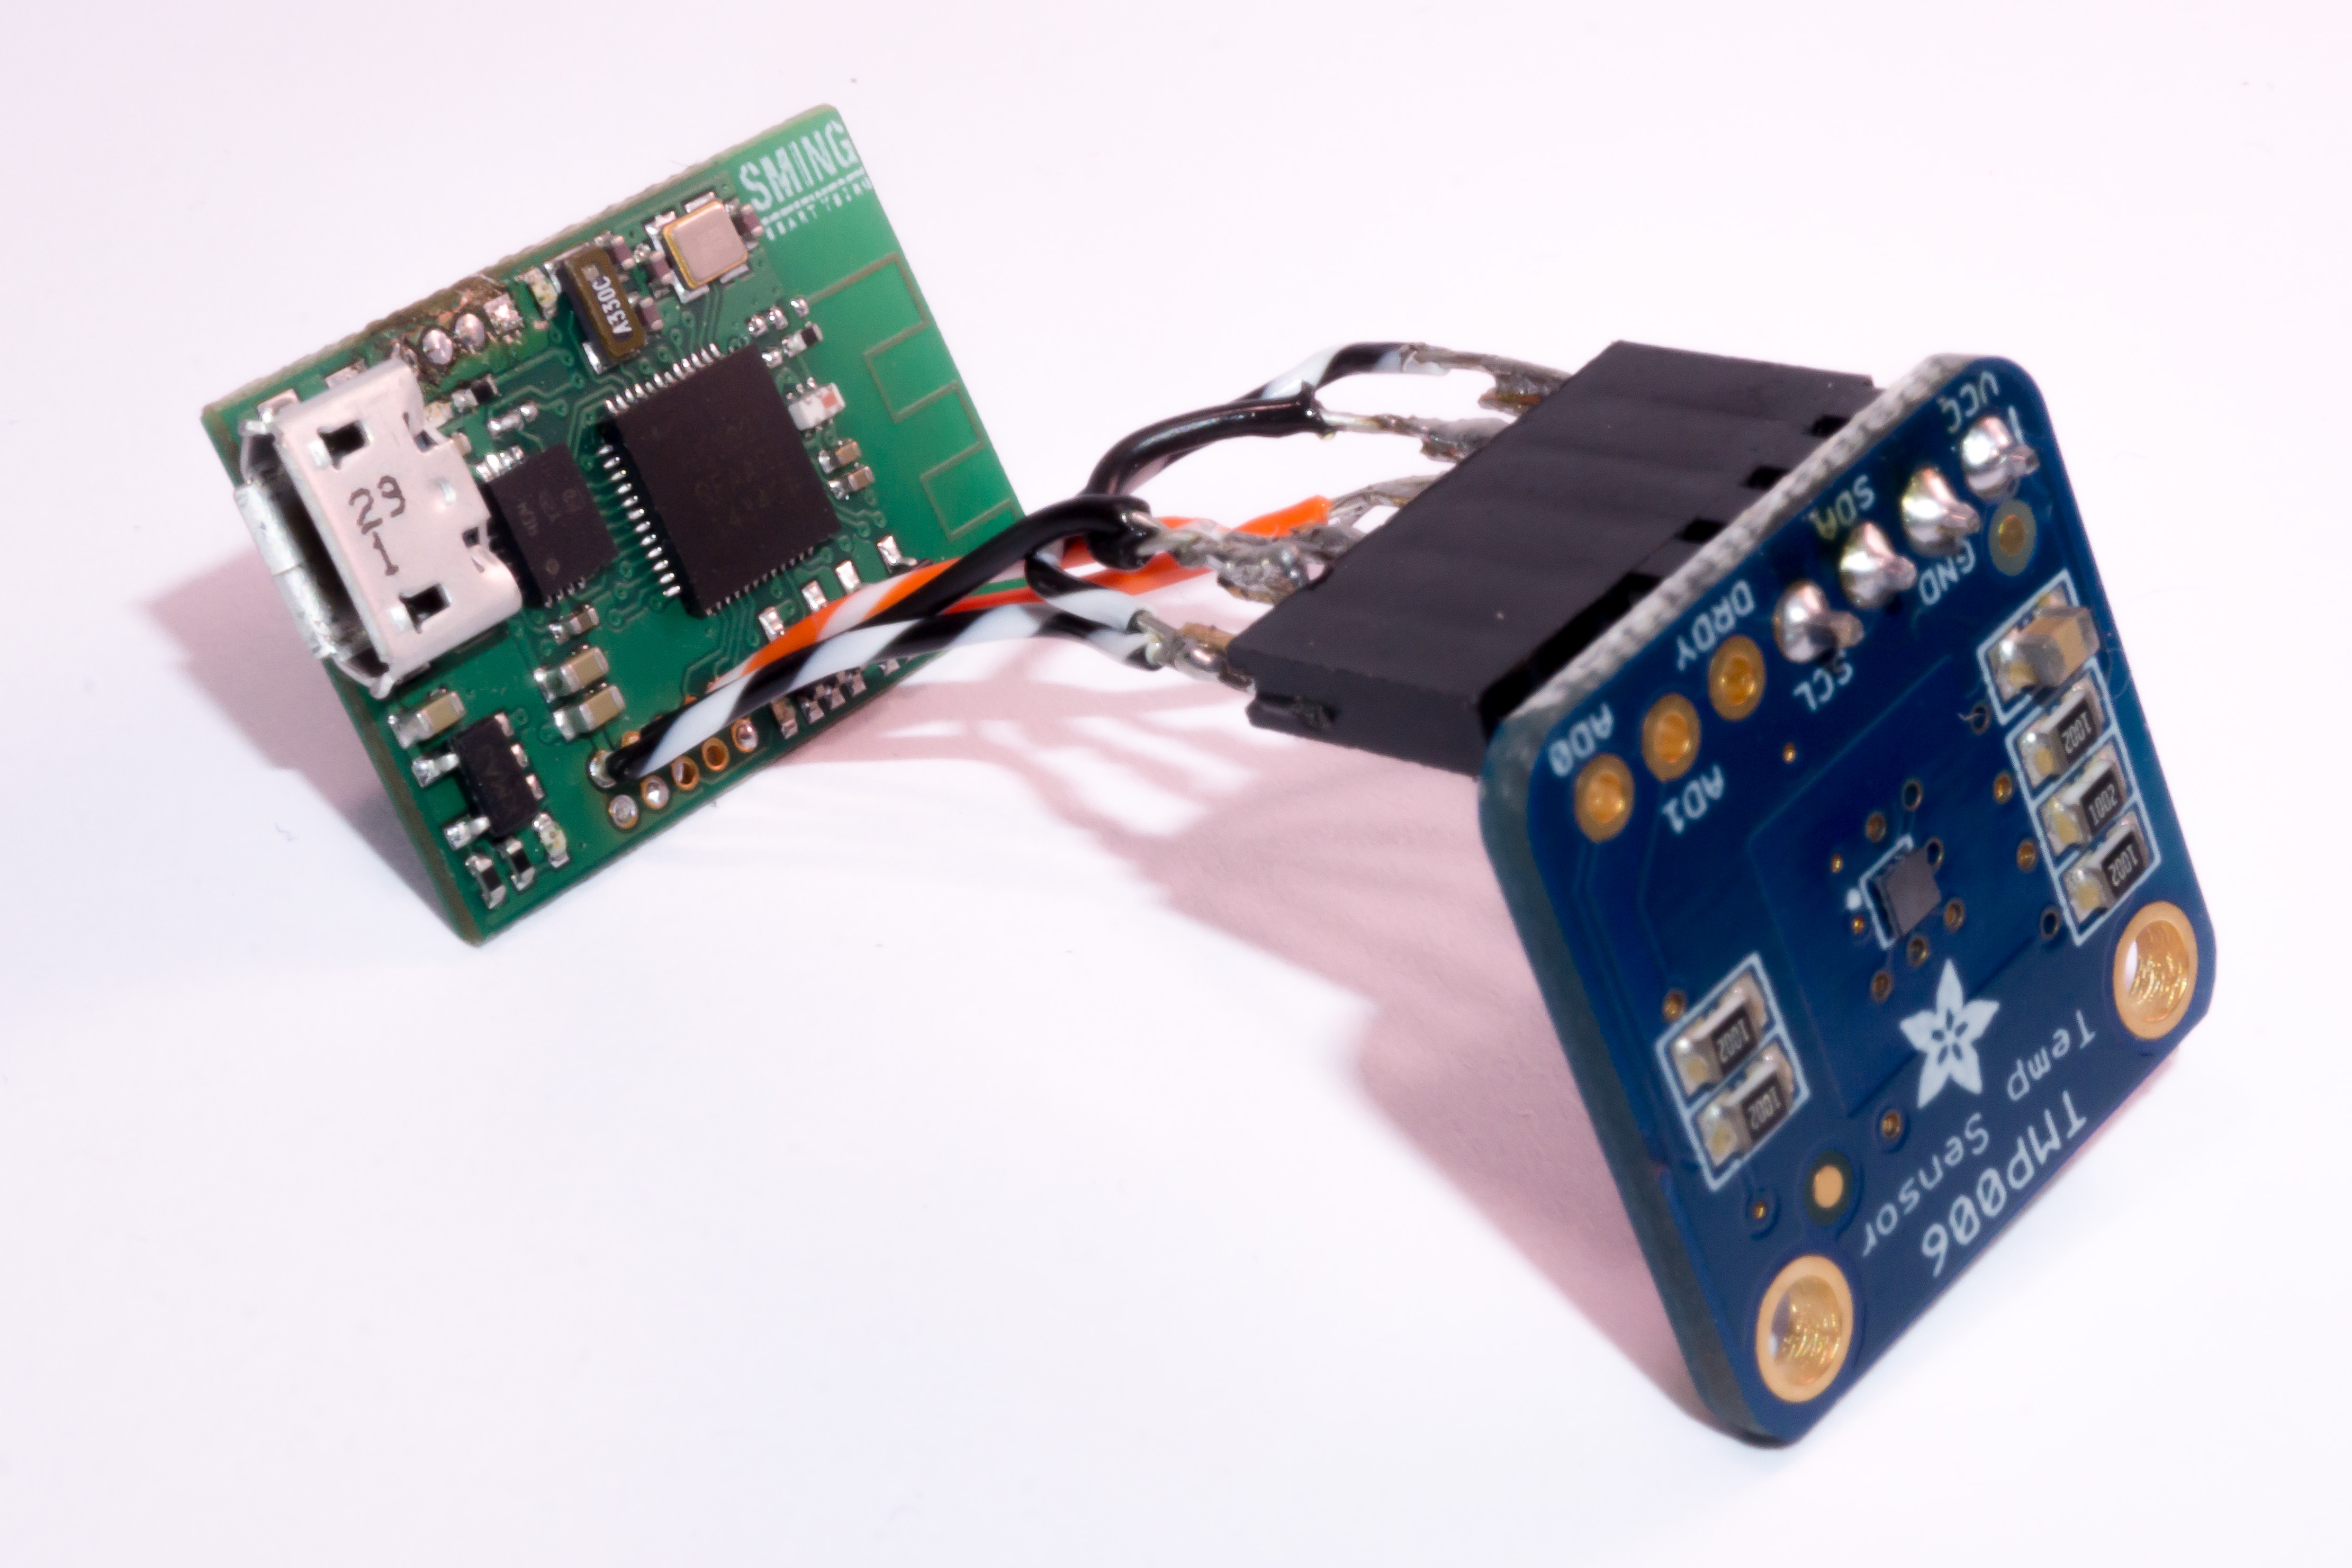
\includegraphics[width=\textwidth]{bilder/foto-2.jpg}
    \caption{Sming mit über I2C Bridge abfragbaren TMP06 Sensor}
    \label{fig:sming_mit_tmp06}
\end{figure}


\section{Implementation}
\label{bleI2cImplementation}

Für die BLE-I2C Bridge wurde ein eigener BLE-Service aufgesetzt.

%\begin{table}[h]
%\centering
\begin{tabularx}{\textwidth}{|l|X|}
\hline
Name & I2C Service                                       \\
\hline
Beschreibung & Ein Service für I2C Devices über BLE anzusprechen \\
\hline
UUID	&    0x8EDF0500-67E5-DB83-F85B-A1E2AB1C9E7A  \\
\hline                                            
\end{tabularx}
%\caption{Ble I2C Service}
%\label{tab:bleI2cService}
%\end{table}

folgende Charakteristiken stehen bei diesem Service zur Verfügung:

%\begin{table}[h]
%\centering
\begin{tabularx}{\textwidth}{|l|X|}
\hline
Name & I2C Device Adress                                   \\
\hline
Beschreibung & Wird verwendet um die I2C Adresse des Sensor (oder Aktor) im Sming einzustellen. \\
\hline
UUID	&    0x8EDF0501-67E5-DB83-F85B-A1E2AB1C9E7A  \\
\hline     
Anzahl Byte	&    1  \\
\hline      
Zugriffsrechte	&   R/W  \\
\hline        
Wertebereich	&   0x00 .. 0x7F \\
\hline          
Wertebereich	&   0x00 \\
\hline                                     
\end{tabularx}
%\caption{Ble I2C Device Adress Charakteristik}
%\label{tab:bleI2cDeviceAdress}
%\end{table}

%\begin{table}[h]
%\centering
\begin{tabularx}{\textwidth}{|l|X|}
\hline
Name & I2C Device Register                                  \\
\hline
Beschreibung & Wird verwendet um das I2C Register des Sensor (oder Aktor) im Sming einzustellen, auf welches geschrieben oder von welchem gelesen werden soll. \\
\hline
UUID	&    0x8EDF0502-67E5-DB83-F85B-A1E2AB1C9E7A  \\
\hline     
Anzahl Byte	&    1  \\
\hline      
Zugriffsrechte	&   R/W  \\
\hline        
Wertebereich	&   0x00 .. 0xFF \\
\hline          
Wertebereich	&   0x00 \\
\hline                                     
\end{tabularx}
%\caption{Ble I2C Device Register Charakteristik}
%\label{tab:bleI2cDeviceRegister}
%\end{table}

%\begin{table}[h]
%\centering
\begin{tabularx}{\textwidth}{|l|X|}
\hline
Name & I2C Read Length                              \\
\hline
Beschreibung & Wird verwendet um die Anzahl Bytes einzustellen, welche von dem eingestellten Register gelesen werden. \\
\hline
UUID	&    0x8EDF0503-67E5-DB83-F85B-A1E2AB1C9E7A \\
\hline     
Anzahl Byte	&    1  \\
\hline      
Zugriffsrechte	&   R/W  \\
\hline        
Wertebereich	&   0x00 .. 0xFF \\
\hline          
Wertebereich	&   0x00 \\
\hline                                     
\end{tabularx}
%\caption{Ble I2C Device Read Length Charakteristik}
%\label{tab:bleI2cDeviceReadLength}
%\end{table}

%\begin{table}[h]
%\centering
\begin{tabularx}{\textwidth}{|l|X|}
\hline
Name & I2C Read Length                              \\
\hline
Beschreibung & Wird verwendet um die eingestellte Anzahl Bytes von dem eingestellten Register zu lesen oder die in der Charakteristik mitgegebene Anzahl Bytes auf das angegebene Register zu schreiben.\\
\hline
UUID	&    0x8EDF0504-67E5-DB83-F85B-A1E2AB1C9E7A \\
\hline     
Anzahl Byte	&    1 .. 10  \\
\hline      
Zugriffsrechte	&   R/W  \\
\hline        
Wertebereich	&   0x00 .. 0xFF \\
\hline          
Wertebereich	&   0x00 \\
\hline                                     
\end{tabularx}
%\caption{Ble I2C Value Charakteristik}
%\label{tab:bleI2cValue}
%\end{table}